\documentclass[1p]{elsarticle_modified}
%\bibliographystyle{elsarticle-num}

%\usepackage[colorlinks]{hyperref}
%\usepackage{abbrmath_seonhwa} %\Abb, \Ascr, \Acal ,\Abf, \Afrak
\usepackage{amsfonts}
\usepackage{amssymb}
\usepackage{amsmath}
\usepackage{amsthm}
\usepackage{scalefnt}
\usepackage{amsbsy}
\usepackage{kotex}
\usepackage{caption}
\usepackage{subfig}
\usepackage{color}
\usepackage{graphicx}
\usepackage{xcolor} %% white, black, red, green, blue, cyan, magenta, yellow
\usepackage{float}
\usepackage{setspace}
\usepackage{hyperref}

\usepackage{tikz}
\usetikzlibrary{arrows}

\usepackage{multirow}
\usepackage{array} % fixed length table
\usepackage{hhline}

%%%%%%%%%%%%%%%%%%%%%
\makeatletter
\renewcommand*\env@matrix[1][\arraystretch]{%
	\edef\arraystretch{#1}%
	\hskip -\arraycolsep
	\let\@ifnextchar\new@ifnextchar
	\array{*\c@MaxMatrixCols c}}
\makeatother %https://tex.stackexchange.com/questions/14071/how-can-i-increase-the-line-spacing-in-a-matrix
%%%%%%%%%%%%%%%

\usepackage[normalem]{ulem}

\newcommand{\msout}[1]{\ifmmode\text{\sout{\ensuremath{#1}}}\else\sout{#1}\fi}
%SOURCE: \msout is \stkout macro in https://tex.stackexchange.com/questions/20609/strikeout-in-math-mode

\newcommand{\cancel}[1]{
	\ifmmode
	{\color{red}\msout{#1}}
	\else
	{\color{red}\sout{#1}}
	\fi
}

\newcommand{\add}[1]{
	{\color{blue}\uwave{#1}}
}

\newcommand{\replace}[2]{
	\ifmmode
	{\color{red}\msout{#1}}{\color{blue}\uwave{#2}}
	\else
	{\color{red}\sout{#1}}{\color{blue}\uwave{#2}}
	\fi
}

\newcommand{\Sol}{\mathcal{S}} %segment
\newcommand{\D}{D} %diagram
\newcommand{\A}{\mathcal{A}} %arc


%%%%%%%%%%%%%%%%%%%%%%%%%%%%%5 test

\def\sl{\operatorname{\textup{SL}}(2,\Cbb)}
\def\psl{\operatorname{\textup{PSL}}(2,\Cbb)}
\def\quan{\mkern 1mu \triangleright \mkern 1mu}

\theoremstyle{definition}
\newtheorem{thm}{Theorem}[section]
\newtheorem{prop}[thm]{Proposition}
\newtheorem{lem}[thm]{Lemma}
\newtheorem{ques}[thm]{Question}
\newtheorem{cor}[thm]{Corollary}
\newtheorem{defn}[thm]{Definition}
\newtheorem{exam}[thm]{Example}
\newtheorem{rmk}[thm]{Remark}
\newtheorem{alg}[thm]{Algorithm}

\newcommand{\I}{\sqrt{-1}}
\begin{document}

%\begin{frontmatter}
%
%\title{Boundary parabolic representations of knots up to 8 crossings}
%
%%% Group authors per affiliation:
%\author{Yunhi Cho} 
%\address{Department of Mathematics, University of Seoul, Seoul, Korea}
%\ead{yhcho@uos.ac.kr}
%
%
%\author{Seonhwa Kim} %\fnref{s_kim}}
%\address{Center for Geometry and Physics, Institute for Basic Science, Pohang, 37673, Korea}
%\ead{ryeona17@ibs.re.kr}
%
%\author{Hyuk Kim}
%\address{Department of Mathematical Sciences, Seoul National University, Seoul 08826, Korea}
%\ead{hyukkim@snu.ac.kr}
%
%\author{Seokbeom Yoon}
%\address{Department of Mathematical Sciences, Seoul National University, Seoul, 08826,  Korea}
%\ead{sbyoon15@snu.ac.kr}
%
%\begin{abstract}
%We find all boundary parabolic representation of knots up to 8 crossings.
%
%\end{abstract}
%\begin{keyword}
%    \MSC[2010] 57M25 
%\end{keyword}
%
%\end{frontmatter}

%\linenumbers
%\tableofcontents
%
\newcommand\colored[1]{\textcolor{white}{\rule[-0.35ex]{0.8em}{1.4ex}}\kern-0.8em\color{red} #1}%
%\newcommand\colored[1]{\textcolor{white}{ #1}\kern-2.17ex	\textcolor{white}{ #1}\kern-1.81ex	\textcolor{white}{ #1}\kern-2.15ex\color{red}#1	}

{\Large $\underline{12n_{0702}~(K12n_{0702})}$}

\setlength{\tabcolsep}{10pt}
\renewcommand{\arraystretch}{1.6}
\vspace{1cm}\begin{tabular}{m{100pt}>{\centering\arraybackslash}m{274pt}}
\multirow{5}{120pt}{
	\centering
	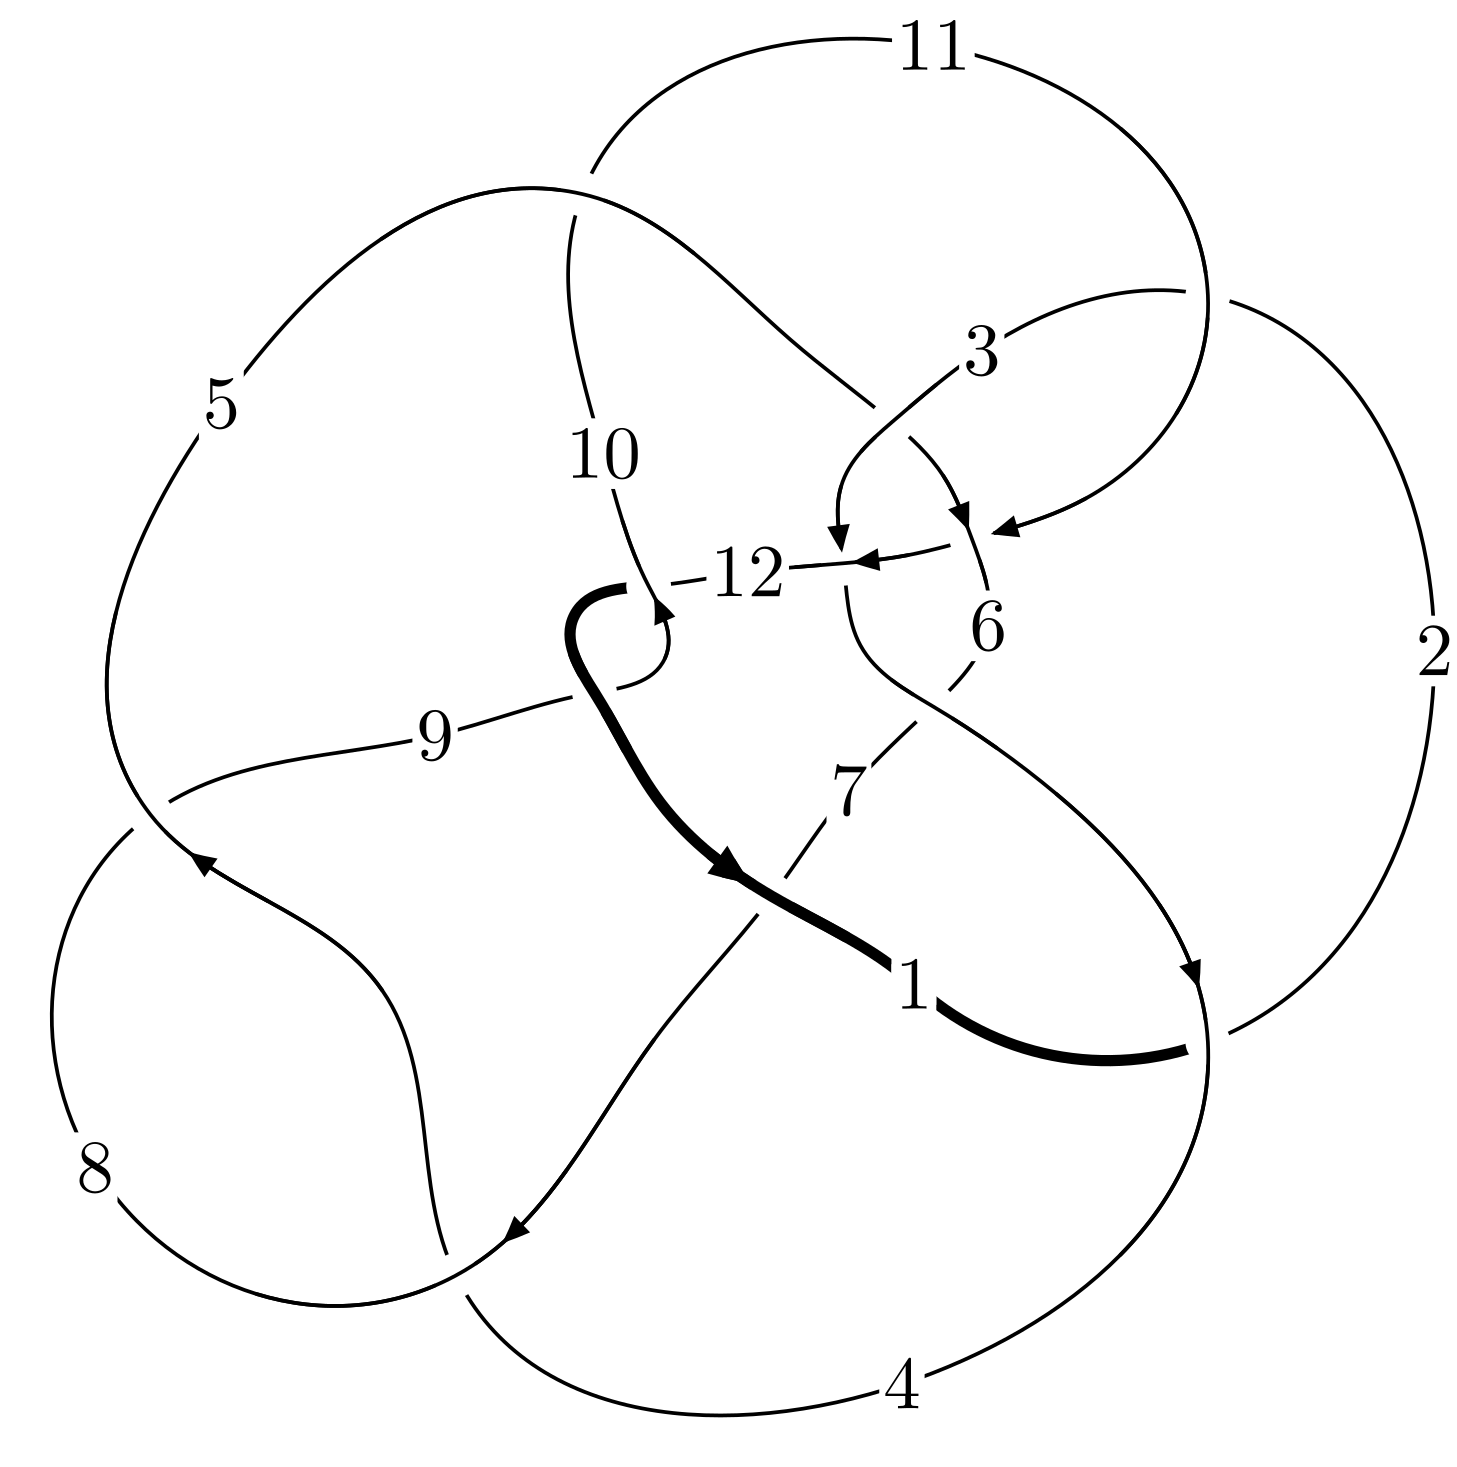
\includegraphics[width=112pt]{../../../GIT/diagram.site/Diagrams/png/2791_12n_0702.png}\\
\ \ \ A knot diagram\footnotemark}&
\allowdisplaybreaks
\textbf{Linearized knot diagam} \\
\cline{2-2}
 &
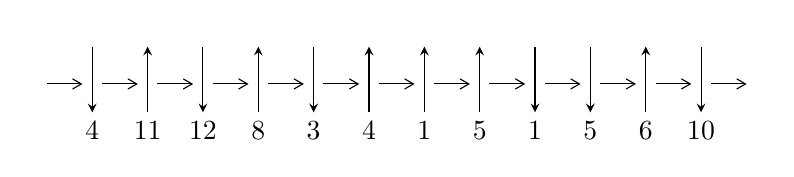
\begin{tikzpicture}[x=20pt, y=17pt]
	% nodes
	\node (C0) at (0, 0) {};
	\node (C1) at (1, 0) {};
	\node (C1U) at (1, +1) {};
	\node (C1D) at (1, -1) {4};

	\node (C2) at (2, 0) {};
	\node (C2U) at (2, +1) {};
	\node (C2D) at (2, -1) {11};

	\node (C3) at (3, 0) {};
	\node (C3U) at (3, +1) {};
	\node (C3D) at (3, -1) {12};

	\node (C4) at (4, 0) {};
	\node (C4U) at (4, +1) {};
	\node (C4D) at (4, -1) {8};

	\node (C5) at (5, 0) {};
	\node (C5U) at (5, +1) {};
	\node (C5D) at (5, -1) {3};

	\node (C6) at (6, 0) {};
	\node (C6U) at (6, +1) {};
	\node (C6D) at (6, -1) {4};

	\node (C7) at (7, 0) {};
	\node (C7U) at (7, +1) {};
	\node (C7D) at (7, -1) {1};

	\node (C8) at (8, 0) {};
	\node (C8U) at (8, +1) {};
	\node (C8D) at (8, -1) {5};

	\node (C9) at (9, 0) {};
	\node (C9U) at (9, +1) {};
	\node (C9D) at (9, -1) {1};

	\node (C10) at (10, 0) {};
	\node (C10U) at (10, +1) {};
	\node (C10D) at (10, -1) {5};

	\node (C11) at (11, 0) {};
	\node (C11U) at (11, +1) {};
	\node (C11D) at (11, -1) {6};

	\node (C12) at (12, 0) {};
	\node (C12U) at (12, +1) {};
	\node (C12D) at (12, -1) {10};
	\node (C13) at (13, 0) {};

	% arrows
	\draw[->,>={angle 60}]
	(C0) edge (C1) (C1) edge (C2) (C2) edge (C3) (C3) edge (C4) (C4) edge (C5) (C5) edge (C6) (C6) edge (C7) (C7) edge (C8) (C8) edge (C9) (C9) edge (C10) (C10) edge (C11) (C11) edge (C12) (C12) edge (C13) ;	\draw[->,>=stealth]
	(C1U) edge (C1D) (C2D) edge (C2U) (C3U) edge (C3D) (C4D) edge (C4U) (C5U) edge (C5D) (C6D) edge (C6U) (C7D) edge (C7U) (C8D) edge (C8U) (C9U) edge (C9D) (C10U) edge (C10D) (C11D) edge (C11U) (C12U) edge (C12D) ;
	\end{tikzpicture} \\
\hhline{~~} \\& 
\textbf{Solving Sequence} \\ \cline{2-2} 
 &
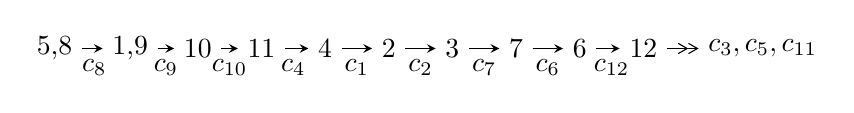
\begin{tikzpicture}[x=23pt, y=7pt]
	% node
	\node (A0) at (-1/8, 0) {5,8};
	\node (A1) at (17/16, 0) {1,9};
	\node (A2) at (17/8, 0) {10};
	\node (A3) at (25/8, 0) {11};
	\node (A4) at (33/8, 0) {4};
	\node (A5) at (41/8, 0) {2};
	\node (A6) at (49/8, 0) {3};
	\node (A7) at (57/8, 0) {7};
	\node (A8) at (65/8, 0) {6};
	\node (A9) at (73/8, 0) {12};
	\node (C1) at (1/2, -1) {$c_{8}$};
	\node (C2) at (13/8, -1) {$c_{9}$};
	\node (C3) at (21/8, -1) {$c_{10}$};
	\node (C4) at (29/8, -1) {$c_{4}$};
	\node (C5) at (37/8, -1) {$c_{1}$};
	\node (C6) at (45/8, -1) {$c_{2}$};
	\node (C7) at (53/8, -1) {$c_{7}$};
	\node (C8) at (61/8, -1) {$c_{6}$};
	\node (C9) at (69/8, -1) {$c_{12}$};
	\node (A10) at (11, 0) {$c_{3},c_{5},c_{11}$};

	% edge
	\draw[->,>=stealth]	
	(A0) edge (A1) (A1) edge (A2) (A2) edge (A3) (A3) edge (A4) (A4) edge (A5) (A5) edge (A6) (A6) edge (A7) (A7) edge (A8) (A8) edge (A9) ;
	\draw[->>,>={angle 60}]	
	(A9) edge (A10);
\end{tikzpicture} \\ 

\end{tabular} \\

\footnotetext{
The image of knot diagram is generated by the software ``\textbf{Draw programme}" developed by Andrew Bartholomew(\url{http://www.layer8.co.uk/maths/draw/index.htm\#Running-draw}), where we modified some parts for our purpose(\url{https://github.com/CATsTAILs/LinksPainter}).
}\phantom \\ \newline 
\centering \textbf{Ideals for irreducible components\footnotemark of $X_{\text{par}}$} 
 
\begin{align*}
I^u_{1}&=\langle 
1.28030\times10^{278} u^{84}-7.08515\times10^{277} u^{83}+\cdots+2.04829\times10^{277} b-1.44299\times10^{278},\\
\phantom{I^u_{1}}&\phantom{= \langle  }-1.59722\times10^{279} u^{84}+5.41005\times10^{278} u^{83}+\cdots+2.04829\times10^{277} a+4.64496\times10^{279},\\
\phantom{I^u_{1}}&\phantom{= \langle  }u^{85}-9 u^{83}+\cdots-8 u-1\rangle \\
I^u_{2}&=\langle 
-244772546 u^{18}-1629957344 u^{17}+\cdots+13743083 b+724816940,\\
\phantom{I^u_{2}}&\phantom{= \langle  }26173603 u^{18}+166772668 u^{17}+\cdots+13743083 a-60671008,\;u^{19}+7 u^{18}+\cdots-8 u-1\rangle \\
I^u_{3}&=\langle 
56 a^5+39 a^4+47 a^3+373 a^2+53 b-362 a-172,\;a^6+a^5+a^4+7 a^3-5 a^2-5 a-1,\;u-1\rangle \\
\\
\end{align*}
\raggedright * 3 irreducible components of $\dim_{\mathbb{C}}=0$, with total 110 representations.\\
\footnotetext{All coefficients of polynomials are rational numbers. But the coefficients are sometimes approximated in decimal forms when there is not enough margin.}
\newpage
\renewcommand{\arraystretch}{1}
\centering \section*{I. $I^u_{1}= \langle 1.28\times10^{278} u^{84}-7.09\times10^{277} u^{83}+\cdots+2.05\times10^{277} b-1.44\times10^{278},\;-1.60\times10^{279} u^{84}+5.41\times10^{278} u^{83}+\cdots+2.05\times10^{277} a+4.64\times10^{279},\;u^{85}-9 u^{83}+\cdots-8 u-1 \rangle$}
\flushleft \textbf{(i) Arc colorings}\\
\begin{tabular}{m{7pt} m{180pt} m{7pt} m{180pt} }
\flushright $a_{5}=$&$\begin{pmatrix}0\\u\end{pmatrix}$ \\
\flushright $a_{8}=$&$\begin{pmatrix}1\\0\end{pmatrix}$ \\
\flushright $a_{1}=$&$\begin{pmatrix}77.9781 u^{84}-26.4125 u^{83}+\cdots-1164.55 u-226.772\\-6.25059 u^{84}+3.45906 u^{83}+\cdots+67.2481 u+7.04483\end{pmatrix}$ \\
\flushright $a_{9}=$&$\begin{pmatrix}1\\- u^2\end{pmatrix}$ \\
\flushright $a_{10}=$&$\begin{pmatrix}-27.5383 u^{84}+8.40815 u^{83}+\cdots+427.301 u+76.0121\\-4.62638 u^{84}+2.16890 u^{83}+\cdots+59.0320 u+6.99337\end{pmatrix}$ \\
\flushright $a_{11}=$&$\begin{pmatrix}-27.5383 u^{84}+8.40815 u^{83}+\cdots+427.301 u+76.0121\\-6.59492 u^{84}+2.34603 u^{83}+\cdots+98.7589 u+15.4015\end{pmatrix}$ \\
\flushright $a_{4}=$&$\begin{pmatrix}- u\\u\end{pmatrix}$ \\
\flushright $a_{2}=$&$\begin{pmatrix}70.9381 u^{84}-24.3526 u^{83}+\cdots-1052.65 u-203.819\\0.789353 u^{84}+1.39912 u^{83}+\cdots-44.6522 u-15.9087\end{pmatrix}$ \\
\flushright $a_{3}=$&$\begin{pmatrix}12.5845 u^{84}-4.95452 u^{83}+\cdots-182.933 u-36.7101\\8.12889 u^{84}-1.77404 u^{83}+\cdots-140.641 u-31.6057\end{pmatrix}$ \\
\flushright $a_{7}=$&$\begin{pmatrix}33.8620 u^{84}-15.4917 u^{83}+\cdots-431.959 u-76.6409\\-11.6733 u^{84}+5.27102 u^{83}+\cdots+149.104 u+22.4851\end{pmatrix}$ \\
\flushright $a_{6}=$&$\begin{pmatrix}29.0802 u^{84}-13.3001 u^{83}+\cdots-372.382 u-66.4202\\-6.89151 u^{84}+3.07940 u^{83}+\cdots+89.5269 u+12.2644\end{pmatrix}$ \\
\flushright $a_{12}=$&$\begin{pmatrix}-0.635360 u^{84}+0.516056 u^{83}+\cdots+4.16244 u-1.48004\\-13.1197 u^{84}+3.93049 u^{83}+\cdots+208.557 u+41.6369\end{pmatrix}$\\&\end{tabular}
\flushleft \textbf{(ii) Obstruction class $= -1$}\\~\\
\flushleft \textbf{(iii) Cusp Shapes $= 16.6730 u^{84}-5.72160 u^{83}+\cdots-248.259 u-50.7302$}\\~\\
\newpage\renewcommand{\arraystretch}{1}
\flushleft \textbf{(iv) u-Polynomials at the component}\newline \\
\begin{tabular}{m{50pt}|m{274pt}}
Crossings & \hspace{64pt}u-Polynomials at each crossing \\
\hline $$\begin{aligned}c_{1}\end{aligned}$$&$\begin{aligned}
&u^{85}+7 u^{84}+\cdots-276406 u-10363
\end{aligned}$\\
\hline $$\begin{aligned}c_{2}\end{aligned}$$&$\begin{aligned}
&u^{85}- u^{84}+\cdots+1536 u-64
\end{aligned}$\\
\hline $$\begin{aligned}c_{3}\end{aligned}$$&$\begin{aligned}
&u^{85}+2 u^{84}+\cdots+4329 u-551
\end{aligned}$\\
\hline $$\begin{aligned}c_{4},c_{8}\end{aligned}$$&$\begin{aligned}
&u^{85}-9 u^{83}+\cdots-8 u-1
\end{aligned}$\\
\hline $$\begin{aligned}c_{5}\end{aligned}$$&$\begin{aligned}
&u^{85}-11 u^{83}+\cdots-9 u-1
\end{aligned}$\\
\hline $$\begin{aligned}c_{6}\end{aligned}$$&$\begin{aligned}
&u^{85}-2 u^{84}+\cdots-2540737042 u-524132531
\end{aligned}$\\
\hline $$\begin{aligned}c_{7}\end{aligned}$$&$\begin{aligned}
&u^{85}+u^{84}+\cdots-35062 u-10369
\end{aligned}$\\
\hline $$\begin{aligned}c_{9},c_{12}\end{aligned}$$&$\begin{aligned}
&u^{85}+4 u^{84}+\cdots+92 u-29
\end{aligned}$\\
\hline $$\begin{aligned}c_{10}\end{aligned}$$&$\begin{aligned}
&u^{85}-26 u^{83}+\cdots-8412115 u-901067
\end{aligned}$\\
\hline $$\begin{aligned}c_{11}\end{aligned}$$&$\begin{aligned}
&u^{85}-4 u^{84}+\cdots-78 u-43
\end{aligned}$\\
\hline
\end{tabular}\\~\\
\newpage\renewcommand{\arraystretch}{1}
\flushleft \textbf{(v) Riley Polynomials at the component}\newline \\
\begin{tabular}{m{50pt}|m{274pt}}
Crossings & \hspace{64pt}Riley Polynomials at each crossing \\
\hline $$\begin{aligned}c_{1}\end{aligned}$$&$\begin{aligned}
&y^{85}-105 y^{84}+\cdots+28067617904 y-107391769
\end{aligned}$\\
\hline $$\begin{aligned}c_{2}\end{aligned}$$&$\begin{aligned}
&y^{85}+43 y^{84}+\cdots+264192 y-4096
\end{aligned}$\\
\hline $$\begin{aligned}c_{3}\end{aligned}$$&$\begin{aligned}
&y^{85}-10 y^{84}+\cdots+13669939 y-303601
\end{aligned}$\\
\hline $$\begin{aligned}c_{4},c_{8}\end{aligned}$$&$\begin{aligned}
&y^{85}-18 y^{84}+\cdots+28 y-1
\end{aligned}$\\
\hline $$\begin{aligned}c_{5}\end{aligned}$$&$\begin{aligned}
&y^{85}-22 y^{84}+\cdots+81 y-1
\end{aligned}$\\
\hline $$\begin{aligned}c_{6}\end{aligned}$$&$\begin{aligned}
&y^{85}+48 y^{84}+\cdots-2812247482606914286 y-274714910052465961
\end{aligned}$\\
\hline $$\begin{aligned}c_{7}\end{aligned}$$&$\begin{aligned}
&y^{85}+69 y^{84}+\cdots+9340452618 y-107516161
\end{aligned}$\\
\hline $$\begin{aligned}c_{9},c_{12}\end{aligned}$$&$\begin{aligned}
&y^{85}+30 y^{84}+\cdots-642 y-841
\end{aligned}$\\
\hline $$\begin{aligned}c_{10}\end{aligned}$$&$\begin{aligned}
&y^{85}-52 y^{84}+\cdots+30213827398679 y-811921738489
\end{aligned}$\\
\hline $$\begin{aligned}c_{11}\end{aligned}$$&$\begin{aligned}
&y^{85}+14 y^{84}+\cdots-59104 y-1849
\end{aligned}$\\
\hline
\end{tabular}\\~\\
\newpage\flushleft \textbf{(vi) Complex Volumes and Cusp Shapes}
$$\begin{array}{c|c|c}  
\text{Solutions to }I^u_{1}& \I (\text{vol} + \sqrt{-1}CS) & \text{Cusp shape}\\
 \hline 
\begin{aligned}
u &= \phantom{-}0.953246 + 0.245682 I \\
a &= \phantom{-}1.007570 - 0.384540 I \\
b &= -0.577244 + 0.241074 I\end{aligned}
 & \phantom{-}0.871396 - 0.259267 I & \phantom{-0.000000 } 0 \\ \hline\begin{aligned}
u &= \phantom{-}0.953246 - 0.245682 I \\
a &= \phantom{-}1.007570 + 0.384540 I \\
b &= -0.577244 - 0.241074 I\end{aligned}
 & \phantom{-}0.871396 + 0.259267 I & \phantom{-0.000000 } 0 \\ \hline\begin{aligned}
u &= -0.673486 + 0.784306 I \\
a &= -1.90573 - 0.56779 I \\
b &= \phantom{-}0.526659 - 1.072070 I\end{aligned}
 & \phantom{-}0.07658 - 7.34708 I & \phantom{-0.000000 } 0 \\ \hline\begin{aligned}
u &= -0.673486 - 0.784306 I \\
a &= -1.90573 + 0.56779 I \\
b &= \phantom{-}0.526659 + 1.072070 I\end{aligned}
 & \phantom{-}0.07658 + 7.34708 I & \phantom{-0.000000 } 0 \\ \hline\begin{aligned}
u &= -0.900856 + 0.557667 I \\
a &= \phantom{-}1.49030 - 0.10055 I \\
b &= -1.56321 + 0.60214 I\end{aligned}
 & \phantom{-}0.25278 - 10.31380 I & \phantom{-0.000000 } 0 \\ \hline\begin{aligned}
u &= -0.900856 - 0.557667 I \\
a &= \phantom{-}1.49030 + 0.10055 I \\
b &= -1.56321 - 0.60214 I\end{aligned}
 & \phantom{-}0.25278 + 10.31380 I & \phantom{-0.000000 } 0 \\ \hline\begin{aligned}
u &= \phantom{-}0.919304 + 0.040533 I \\
a &= \phantom{-}1.81355 + 0.10649 I \\
b &= -2.22407 - 0.17184 I\end{aligned}
 & \phantom{-}0.592523 - 0.002741 I & \phantom{-0.000000 } 0 \\ \hline\begin{aligned}
u &= \phantom{-}0.919304 - 0.040533 I \\
a &= \phantom{-}1.81355 - 0.10649 I \\
b &= -2.22407 + 0.17184 I\end{aligned}
 & \phantom{-}0.592523 + 0.002741 I & \phantom{-0.000000 } 0 \\ \hline\begin{aligned}
u &= -0.748567 + 0.471981 I \\
a &= -1.44360 + 0.65462 I \\
b &= \phantom{-}0.660672 - 0.096154 I\end{aligned}
 & \phantom{-}0.76529 - 4.87151 I & \phantom{-0.000000 } 0 \\ \hline\begin{aligned}
u &= -0.748567 - 0.471981 I \\
a &= -1.44360 - 0.65462 I \\
b &= \phantom{-}0.660672 + 0.096154 I\end{aligned}
 & \phantom{-}0.76529 + 4.87151 I & \phantom{-0.000000 } 0\\
 \hline 
 \end{array}$$\newpage$$\begin{array}{c|c|c}  
\text{Solutions to }I^u_{1}& \I (\text{vol} + \sqrt{-1}CS) & \text{Cusp shape}\\
 \hline 
\begin{aligned}
u &= \phantom{-}1.125640 + 0.071155 I \\
a &= \phantom{-}0.47625 + 1.55494 I \\
b &= -0.071839 - 0.716689 I\end{aligned}
 & \phantom{-}4.27813 - 3.12428 I & \phantom{-0.000000 } 0 \\ \hline\begin{aligned}
u &= \phantom{-}1.125640 - 0.071155 I \\
a &= \phantom{-}0.47625 - 1.55494 I \\
b &= -0.071839 + 0.716689 I\end{aligned}
 & \phantom{-}4.27813 + 3.12428 I & \phantom{-0.000000 } 0 \\ \hline\begin{aligned}
u &= \phantom{-}0.909487 + 0.669545 I \\
a &= \phantom{-}1.210390 - 0.046758 I \\
b &= -0.919489 - 0.617999 I\end{aligned}
 & \phantom{-}2.82901 + 2.24291 I & \phantom{-0.000000 } 0 \\ \hline\begin{aligned}
u &= \phantom{-}0.909487 - 0.669545 I \\
a &= \phantom{-}1.210390 + 0.046758 I \\
b &= -0.919489 + 0.617999 I\end{aligned}
 & \phantom{-}2.82901 - 2.24291 I & \phantom{-0.000000 } 0 \\ \hline\begin{aligned}
u &= \phantom{-}0.540941 + 0.640172 I \\
a &= -0.416849 + 0.792144 I \\
b &= \phantom{-}0.705707 - 0.447204 I\end{aligned}
 & \phantom{-}1.89366 + 2.60688 I & \phantom{-}5.20495 - 4.85763 I \\ \hline\begin{aligned}
u &= \phantom{-}0.540941 - 0.640172 I \\
a &= -0.416849 - 0.792144 I \\
b &= \phantom{-}0.705707 + 0.447204 I\end{aligned}
 & \phantom{-}1.89366 - 2.60688 I & \phantom{-}5.20495 + 4.85763 I \\ \hline\begin{aligned}
u &= -0.514416 + 0.658480 I \\
a &= -1.069110 + 0.163561 I \\
b &= \phantom{-}0.743351 + 0.124486 I\end{aligned}
 & -1.88421 - 3.29048 I & -5.94463 + 7.93366 I \\ \hline\begin{aligned}
u &= -0.514416 - 0.658480 I \\
a &= -1.069110 - 0.163561 I \\
b &= \phantom{-}0.743351 - 0.124486 I\end{aligned}
 & -1.88421 + 3.29048 I & -5.94463 - 7.93366 I \\ \hline\begin{aligned}
u &= -0.110753 + 0.800469 I \\
a &= \phantom{-}1.66054 + 0.49068 I \\
b &= \phantom{-}0.327175 + 0.029384 I\end{aligned}
 & -2.81942 + 2.04516 I & -6.43659 - 2.51371 I \\ \hline\begin{aligned}
u &= -0.110753 - 0.800469 I \\
a &= \phantom{-}1.66054 - 0.49068 I \\
b &= \phantom{-}0.327175 - 0.029384 I\end{aligned}
 & -2.81942 - 2.04516 I & -6.43659 + 2.51371 I\\
 \hline 
 \end{array}$$\newpage$$\begin{array}{c|c|c}  
\text{Solutions to }I^u_{1}& \I (\text{vol} + \sqrt{-1}CS) & \text{Cusp shape}\\
 \hline 
\begin{aligned}
u &= \phantom{-}0.446712 + 0.616825 I \\
a &= -1.39986 + 0.44963 I \\
b &= \phantom{-}0.903744 - 0.202836 I\end{aligned}
 & -1.11341 + 3.76827 I & -7.97957 - 5.72070 I \\ \hline\begin{aligned}
u &= \phantom{-}0.446712 - 0.616825 I \\
a &= -1.39986 - 0.44963 I \\
b &= \phantom{-}0.903744 + 0.202836 I\end{aligned}
 & -1.11341 - 3.76827 I & -7.97957 + 5.72070 I \\ \hline\begin{aligned}
u &= \phantom{-}0.022513 + 0.738228 I \\
a &= \phantom{-}1.98080 - 1.09389 I \\
b &= \phantom{-}0.520976 + 0.287420 I\end{aligned}
 & -1.68094 + 6.59296 I & -4.00324 - 6.24155 I \\ \hline\begin{aligned}
u &= \phantom{-}0.022513 - 0.738228 I \\
a &= \phantom{-}1.98080 + 1.09389 I \\
b &= \phantom{-}0.520976 - 0.287420 I\end{aligned}
 & -1.68094 - 6.59296 I & -4.00324 + 6.24155 I \\ \hline\begin{aligned}
u &= -0.987717 + 0.803260 I \\
a &= \phantom{-}1.045390 - 0.151570 I \\
b &= -0.259808 + 1.320130 I\end{aligned}
 & -2.86081 - 2.98975 I & \phantom{-0.000000 } 0 \\ \hline\begin{aligned}
u &= -0.987717 - 0.803260 I \\
a &= \phantom{-}1.045390 + 0.151570 I \\
b &= -0.259808 - 1.320130 I\end{aligned}
 & -2.86081 + 2.98975 I & \phantom{-0.000000 } 0 \\ \hline\begin{aligned}
u &= -0.074158 + 1.272450 I \\
a &= \phantom{-}0.230434 + 0.820563 I \\
b &= \phantom{-}0.235221 + 0.844978 I\end{aligned}
 & -3.68207 + 0.90101 I & \phantom{-0.000000 } 0 \\ \hline\begin{aligned}
u &= -0.074158 - 1.272450 I \\
a &= \phantom{-}0.230434 - 0.820563 I \\
b &= \phantom{-}0.235221 - 0.844978 I\end{aligned}
 & -3.68207 - 0.90101 I & \phantom{-0.000000 } 0 \\ \hline\begin{aligned}
u &= -0.778773 + 1.013300 I \\
a &= -0.811119 + 0.504897 I \\
b &= \phantom{-}0.24015 - 1.57375 I\end{aligned}
 & -7.82081 - 0.90724 I & \phantom{-0.000000 } 0 \\ \hline\begin{aligned}
u &= -0.778773 - 1.013300 I \\
a &= -0.811119 - 0.504897 I \\
b &= \phantom{-}0.24015 + 1.57375 I\end{aligned}
 & -7.82081 + 0.90724 I & \phantom{-0.000000 } 0\\
 \hline 
 \end{array}$$\newpage$$\begin{array}{c|c|c}  
\text{Solutions to }I^u_{1}& \I (\text{vol} + \sqrt{-1}CS) & \text{Cusp shape}\\
 \hline 
\begin{aligned}
u &= \phantom{-}0.717565\phantom{ +0.000000I} \\
a &= \phantom{-}1.09859\phantom{ +0.000000I} \\
b &= -0.748487\phantom{ +0.000000I}\end{aligned}
 & \phantom{-}1.23485\phantom{ +0.000000I} & \phantom{-}8.37230\phantom{ +0.000000I} \\ \hline\begin{aligned}
u &= -1.275380 + 0.256516 I \\
a &= -0.200937 + 0.717636 I \\
b &= -0.163799 + 0.011266 I\end{aligned}
 & \phantom{-}6.70429 - 4.67725 I & \phantom{-0.000000 } 0 \\ \hline\begin{aligned}
u &= -1.275380 - 0.256516 I \\
a &= -0.200937 - 0.717636 I \\
b &= -0.163799 - 0.011266 I\end{aligned}
 & \phantom{-}6.70429 + 4.67725 I & \phantom{-0.000000 } 0 \\ \hline\begin{aligned}
u &= -0.861322 + 0.988040 I \\
a &= \phantom{-}0.626308 - 0.287592 I \\
b &= -0.30284 + 1.82816 I\end{aligned}
 & -6.97709 - 2.44068 I & \phantom{-0.000000 } 0 \\ \hline\begin{aligned}
u &= -0.861322 - 0.988040 I \\
a &= \phantom{-}0.626308 + 0.287592 I \\
b &= -0.30284 - 1.82816 I\end{aligned}
 & -6.97709 + 2.44068 I & \phantom{-0.000000 } 0 \\ \hline\begin{aligned}
u &= \phantom{-}0.671632 + 0.108498 I \\
a &= -3.18695 - 0.42608 I \\
b &= \phantom{-}1.76184 + 0.45532 I\end{aligned}
 & -0.629345 + 0.042189 I & -9.3237 - 22.9586 I \\ \hline\begin{aligned}
u &= \phantom{-}0.671632 - 0.108498 I \\
a &= -3.18695 + 0.42608 I \\
b &= \phantom{-}1.76184 - 0.45532 I\end{aligned}
 & -0.629345 - 0.042189 I & -9.3237 + 22.9586 I \\ \hline\begin{aligned}
u &= \phantom{-}1.320680 + 0.030383 I \\
a &= \phantom{-}0.374873 + 0.695666 I \\
b &= -0.439824 - 0.683093 I\end{aligned}
 & \phantom{-}2.63381 - 0.38628 I & \phantom{-0.000000 } 0 \\ \hline\begin{aligned}
u &= \phantom{-}1.320680 - 0.030383 I \\
a &= \phantom{-}0.374873 - 0.695666 I \\
b &= -0.439824 + 0.683093 I\end{aligned}
 & \phantom{-}2.63381 + 0.38628 I & \phantom{-0.000000 } 0 \\ \hline\begin{aligned}
u &= \phantom{-}1.328070 + 0.070537 I \\
a &= \phantom{-}0.209036 - 0.094466 I \\
b &= -0.680596 - 0.890239 I\end{aligned}
 & \phantom{-}3.43139 - 3.10183 I & \phantom{-0.000000 } 0\\
 \hline 
 \end{array}$$\newpage$$\begin{array}{c|c|c}  
\text{Solutions to }I^u_{1}& \I (\text{vol} + \sqrt{-1}CS) & \text{Cusp shape}\\
 \hline 
\begin{aligned}
u &= \phantom{-}1.328070 - 0.070537 I \\
a &= \phantom{-}0.209036 + 0.094466 I \\
b &= -0.680596 + 0.890239 I\end{aligned}
 & \phantom{-}3.43139 + 3.10183 I & \phantom{-0.000000 } 0 \\ \hline\begin{aligned}
u &= -0.818817 + 1.054500 I \\
a &= -0.397386 + 0.496106 I \\
b &= \phantom{-}0.01047 - 1.52855 I\end{aligned}
 & -6.06632 + 1.74224 I & \phantom{-0.000000 } 0 \\ \hline\begin{aligned}
u &= -0.818817 - 1.054500 I \\
a &= -0.397386 - 0.496106 I \\
b &= \phantom{-}0.01047 + 1.52855 I\end{aligned}
 & -6.06632 - 1.74224 I & \phantom{-0.000000 } 0 \\ \hline\begin{aligned}
u &= \phantom{-}0.853790 + 1.031930 I \\
a &= \phantom{-}0.702437 + 0.384444 I \\
b &= -0.38963 - 1.74425 I\end{aligned}
 & -8.60891 + 10.06010 I & \phantom{-0.000000 } 0 \\ \hline\begin{aligned}
u &= \phantom{-}0.853790 - 1.031930 I \\
a &= \phantom{-}0.702437 - 0.384444 I \\
b &= -0.38963 + 1.74425 I\end{aligned}
 & -8.60891 - 10.06010 I & \phantom{-0.000000 } 0 \\ \hline\begin{aligned}
u &= \phantom{-}0.569474 + 1.212630 I \\
a &= -0.588783 - 0.156268 I \\
b &= \phantom{-}0.21959 + 1.40637 I\end{aligned}
 & -6.53669 - 0.30535 I & \phantom{-0.000000 } 0 \\ \hline\begin{aligned}
u &= \phantom{-}0.569474 - 1.212630 I \\
a &= -0.588783 + 0.156268 I \\
b &= \phantom{-}0.21959 - 1.40637 I\end{aligned}
 & -6.53669 + 0.30535 I & \phantom{-0.000000 } 0 \\ \hline\begin{aligned}
u &= -0.643333 + 0.126775 I \\
a &= \phantom{-}0.700532 + 0.525270 I \\
b &= -0.86233 - 1.30596 I\end{aligned}
 & \phantom{-}1.11800 + 3.76540 I & \phantom{-}6.47146 - 0.17501 I \\ \hline\begin{aligned}
u &= -0.643333 - 0.126775 I \\
a &= \phantom{-}0.700532 - 0.525270 I \\
b &= -0.86233 + 1.30596 I\end{aligned}
 & \phantom{-}1.11800 - 3.76540 I & \phantom{-}6.47146 + 0.17501 I \\ \hline\begin{aligned}
u &= -1.072820 + 0.880544 I \\
a &= \phantom{-}1.222270 - 0.647004 I \\
b &= \phantom{-}0.06919 + 1.47723 I\end{aligned}
 & -6.28594 - 4.46244 I & \phantom{-0.000000 } 0\\
 \hline 
 \end{array}$$\newpage$$\begin{array}{c|c|c}  
\text{Solutions to }I^u_{1}& \I (\text{vol} + \sqrt{-1}CS) & \text{Cusp shape}\\
 \hline 
\begin{aligned}
u &= -1.072820 - 0.880544 I \\
a &= \phantom{-}1.222270 + 0.647004 I \\
b &= \phantom{-}0.06919 - 1.47723 I\end{aligned}
 & -6.28594 + 4.46244 I & \phantom{-0.000000 } 0 \\ \hline\begin{aligned}
u &= -1.111240 + 0.836819 I \\
a &= -1.085760 + 0.719028 I \\
b &= \phantom{-}0.34024 - 1.57099 I\end{aligned}
 & -6.73268 - 5.90485 I & \phantom{-0.000000 } 0 \\ \hline\begin{aligned}
u &= -1.111240 - 0.836819 I \\
a &= -1.085760 - 0.719028 I \\
b &= \phantom{-}0.34024 + 1.57099 I\end{aligned}
 & -6.73268 + 5.90485 I & \phantom{-0.000000 } 0 \\ \hline\begin{aligned}
u &= -0.597072 + 0.076683 I \\
a &= \phantom{-}0.939533 + 0.529541 I \\
b &= -0.223355 + 1.043000 I\end{aligned}
 & \phantom{-}0.72842 - 3.14108 I & \phantom{-}2.29680 + 4.43516 I \\ \hline\begin{aligned}
u &= -0.597072 - 0.076683 I \\
a &= \phantom{-}0.939533 - 0.529541 I \\
b &= -0.223355 - 1.043000 I\end{aligned}
 & \phantom{-}0.72842 + 3.14108 I & \phantom{-}2.29680 - 4.43516 I \\ \hline\begin{aligned}
u &= -1.10536 + 0.91023 I \\
a &= -1.277440 + 0.468808 I \\
b &= \phantom{-}0.45655 - 1.40048 I\end{aligned}
 & -5.15199 - 8.90397 I & \phantom{-0.000000 } 0 \\ \hline\begin{aligned}
u &= -1.10536 - 0.91023 I \\
a &= -1.277440 - 0.468808 I \\
b &= \phantom{-}0.45655 + 1.40048 I\end{aligned}
 & -5.15199 + 8.90397 I & \phantom{-0.000000 } 0 \\ \hline\begin{aligned}
u &= -0.83913 + 1.17729 I \\
a &= \phantom{-}0.532658 - 0.417502 I \\
b &= \phantom{-}0.35403 + 1.48319 I\end{aligned}
 & -7.44292 + 1.34945 I & \phantom{-0.000000 } 0 \\ \hline\begin{aligned}
u &= -0.83913 - 1.17729 I \\
a &= \phantom{-}0.532658 + 0.417502 I \\
b &= \phantom{-}0.35403 - 1.48319 I\end{aligned}
 & -7.44292 - 1.34945 I & \phantom{-0.000000 } 0 \\ \hline\begin{aligned}
u &= \phantom{-}1.12975 + 0.91492 I \\
a &= \phantom{-}1.007260 + 0.695928 I \\
b &= \phantom{-}0.02880 - 1.41413 I\end{aligned}
 & -7.74485 - 2.88977 I & \phantom{-0.000000 } 0\\
 \hline 
 \end{array}$$\newpage$$\begin{array}{c|c|c}  
\text{Solutions to }I^u_{1}& \I (\text{vol} + \sqrt{-1}CS) & \text{Cusp shape}\\
 \hline 
\begin{aligned}
u &= \phantom{-}1.12975 - 0.91492 I \\
a &= \phantom{-}1.007260 - 0.695928 I \\
b &= \phantom{-}0.02880 + 1.41413 I\end{aligned}
 & -7.74485 + 2.88977 I & \phantom{-0.000000 } 0 \\ \hline\begin{aligned}
u &= \phantom{-}0.82642 + 1.24387 I \\
a &= \phantom{-}0.435680 + 0.402752 I \\
b &= \phantom{-}0.26320 - 1.49705 I\end{aligned}
 & -7.78575 - 9.87450 I & \phantom{-0.000000 } 0 \\ \hline\begin{aligned}
u &= \phantom{-}0.82642 - 1.24387 I \\
a &= \phantom{-}0.435680 - 0.402752 I \\
b &= \phantom{-}0.26320 + 1.49705 I\end{aligned}
 & -7.78575 + 9.87450 I & \phantom{-0.000000 } 0 \\ \hline\begin{aligned}
u &= -1.16879 + 0.95091 I \\
a &= \phantom{-}1.168270 - 0.342096 I \\
b &= -0.62166 + 1.72667 I\end{aligned}
 & -6.33003 - 9.02103 I & \phantom{-0.000000 } 0 \\ \hline\begin{aligned}
u &= -1.16879 - 0.95091 I \\
a &= \phantom{-}1.168270 + 0.342096 I \\
b &= -0.62166 - 1.72667 I\end{aligned}
 & -6.33003 + 9.02103 I & \phantom{-0.000000 } 0 \\ \hline\begin{aligned}
u &= \phantom{-}1.18792 + 0.96818 I \\
a &= \phantom{-}1.189930 + 0.382393 I \\
b &= -0.56609 - 1.65671 I\end{aligned}
 & -6.5605 + 17.7584 I & \phantom{-0.000000 } 0 \\ \hline\begin{aligned}
u &= \phantom{-}1.18792 - 0.96818 I \\
a &= \phantom{-}1.189930 - 0.382393 I \\
b &= -0.56609 + 1.65671 I\end{aligned}
 & -6.5605 - 17.7584 I & \phantom{-0.000000 } 0 \\ \hline\begin{aligned}
u &= \phantom{-}0.91255 + 1.27572 I \\
a &= -0.413886 - 0.234512 I \\
b &= \phantom{-}0.090108 + 1.345540 I\end{aligned}
 & -6.23718 + 1.43490 I & \phantom{-0.000000 } 0 \\ \hline\begin{aligned}
u &= \phantom{-}0.91255 - 1.27572 I \\
a &= -0.413886 + 0.234512 I \\
b &= \phantom{-}0.090108 - 1.345540 I\end{aligned}
 & -6.23718 - 1.43490 I & \phantom{-0.000000 } 0 \\ \hline\begin{aligned}
u &= -0.267578 + 0.313151 I \\
a &= \phantom{-}0.055433 + 1.389690 I \\
b &= \phantom{-}0.473363 - 0.261089 I\end{aligned}
 & -1.67196 + 0.33811 I & -4.53587 + 0.25356 I\\
 \hline 
 \end{array}$$\newpage$$\begin{array}{c|c|c}  
\text{Solutions to }I^u_{1}& \I (\text{vol} + \sqrt{-1}CS) & \text{Cusp shape}\\
 \hline 
\begin{aligned}
u &= -0.267578 - 0.313151 I \\
a &= \phantom{-}0.055433 - 1.389690 I \\
b &= \phantom{-}0.473363 + 0.261089 I\end{aligned}
 & -1.67196 - 0.33811 I & -4.53587 - 0.25356 I \\ \hline\begin{aligned}
u &= \phantom{-}1.12120 + 1.13735 I \\
a &= -0.935373 - 0.230456 I \\
b &= \phantom{-}0.317137 + 1.296190 I\end{aligned}
 & -5.58721 + 7.04673 I & \phantom{-0.000000 } 0 \\ \hline\begin{aligned}
u &= \phantom{-}1.12120 - 1.13735 I \\
a &= -0.935373 + 0.230456 I \\
b &= \phantom{-}0.317137 - 1.296190 I\end{aligned}
 & -5.58721 - 7.04673 I & \phantom{-0.000000 } 0 \\ \hline\begin{aligned}
u &= \phantom{-}0.252248 + 0.310284 I \\
a &= -0.838985 - 0.037082 I \\
b &= \phantom{-}0.08832 - 1.69651 I\end{aligned}
 & \phantom{-}1.02683 + 4.68860 I & -4.5379 - 18.7431 I \\ \hline\begin{aligned}
u &= \phantom{-}0.252248 - 0.310284 I \\
a &= -0.838985 + 0.037082 I \\
b &= \phantom{-}0.08832 + 1.69651 I\end{aligned}
 & \phantom{-}1.02683 - 4.68860 I & -4.5379 + 18.7431 I \\ \hline\begin{aligned}
u &= -0.390454 + 0.064131 I \\
a &= -4.96384 - 2.92768 I \\
b &= \phantom{-}0.693941 + 0.917998 I\end{aligned}
 & -1.33214 + 7.02424 I & \phantom{-}1.83651 - 1.94021 I \\ \hline\begin{aligned}
u &= -0.390454 - 0.064131 I \\
a &= -4.96384 + 2.92768 I \\
b &= \phantom{-}0.693941 - 0.917998 I\end{aligned}
 & -1.33214 - 7.02424 I & \phantom{-}1.83651 + 1.94021 I \\ \hline\begin{aligned}
u &= \phantom{-}1.31679 + 0.93534 I \\
a &= -0.877200 - 0.537108 I \\
b &= \phantom{-}0.24804 + 1.41028 I\end{aligned}
 & -4.27143 + 8.08431 I & \phantom{-0.000000 } 0 \\ \hline\begin{aligned}
u &= \phantom{-}1.31679 - 0.93534 I \\
a &= -0.877200 + 0.537108 I \\
b &= \phantom{-}0.24804 - 1.41028 I\end{aligned}
 & -4.27143 - 8.08431 I & \phantom{-0.000000 } 0 \\ \hline\begin{aligned}
u &= -1.64898 + 0.16129 I \\
a &= \phantom{-}0.084326 - 0.476991 I \\
b &= -0.207238 + 0.939937 I\end{aligned}
 & \phantom{-}3.05653 - 5.84434 I & \phantom{-0.000000 } 0\\
 \hline 
 \end{array}$$\newpage$$\begin{array}{c|c|c}  
\text{Solutions to }I^u_{1}& \I (\text{vol} + \sqrt{-1}CS) & \text{Cusp shape}\\
 \hline 
\begin{aligned}
u &= -1.64898 - 0.16129 I \\
a &= \phantom{-}0.084326 + 0.476991 I \\
b &= -0.207238 - 0.939937 I\end{aligned}
 & \phantom{-}3.05653 + 5.84434 I & \phantom{-0.000000 } 0 \\ \hline\begin{aligned}
u &= -0.312911 + 0.076595 I \\
a &= \phantom{-}1.31072 - 3.31226 I \\
b &= \phantom{-}0.225604 - 0.993144 I\end{aligned}
 & \phantom{-}3.12290 + 2.74721 I & \phantom{-}1.20418 - 2.40059 I \\ \hline\begin{aligned}
u &= -0.312911 - 0.076595 I \\
a &= \phantom{-}1.31072 + 3.31226 I \\
b &= \phantom{-}0.225604 + 0.993144 I\end{aligned}
 & \phantom{-}3.12290 - 2.74721 I & \phantom{-}1.20418 + 2.40059 I \\ \hline\begin{aligned}
u &= \phantom{-}0.134773 + 0.261504 I \\
a &= -2.21098 + 3.95237 I \\
b &= \phantom{-}0.443171 + 1.057770 I\end{aligned}
 & -2.30070 - 0.22946 I & -0.69908 + 2.57896 I \\ \hline\begin{aligned}
u &= \phantom{-}0.134773 - 0.261504 I \\
a &= -2.21098 - 3.95237 I \\
b &= \phantom{-}0.443171 - 1.057770 I\end{aligned}
 & -2.30070 + 0.22946 I & -0.69908 - 2.57896 I\\
 \hline 
 \end{array}$$\newpage\newpage\renewcommand{\arraystretch}{1}
\centering \section*{II. $I^u_{2}= \langle -2.45\times10^{8} u^{18}-1.63\times10^{9} u^{17}+\cdots+1.37\times10^{7} b+7.25\times10^{8},\;2.62\times10^{7} u^{18}+1.67\times10^{8} u^{17}+\cdots+1.37\times10^{7} a-6.07\times10^{7},\;u^{19}+7 u^{18}+\cdots-8 u-1 \rangle$}
\flushleft \textbf{(i) Arc colorings}\\
\begin{tabular}{m{7pt} m{180pt} m{7pt} m{180pt} }
\flushright $a_{5}=$&$\begin{pmatrix}0\\u\end{pmatrix}$ \\
\flushright $a_{8}=$&$\begin{pmatrix}1\\0\end{pmatrix}$ \\
\flushright $a_{1}=$&$\begin{pmatrix}-1.90449 u^{18}-12.1350 u^{17}+\cdots+17.7714 u+4.41466\\17.8106 u^{18}+118.602 u^{17}+\cdots-265.643 u-52.7405\end{pmatrix}$ \\
\flushright $a_{9}=$&$\begin{pmatrix}1\\- u^2\end{pmatrix}$ \\
\flushright $a_{10}=$&$\begin{pmatrix}25.9870 u^{18}+172.460 u^{17}+\cdots-380.519 u-74.9910\\-8.44948 u^{18}-55.4779 u^{17}+\cdots+109.905 u+17.9870\end{pmatrix}$ \\
\flushright $a_{11}=$&$\begin{pmatrix}25.9870 u^{18}+172.460 u^{17}+\cdots-380.519 u-74.9910\\-4.78098 u^{18}-31.1791 u^{17}+\cdots+60.2962 u+8.53752\end{pmatrix}$ \\
\flushright $a_{4}=$&$\begin{pmatrix}- u\\u\end{pmatrix}$ \\
\flushright $a_{2}=$&$\begin{pmatrix}-3.40312 u^{18}-22.0099 u^{17}+\cdots+40.8714 u+9.29041\\19.3092 u^{18}+128.477 u^{17}+\cdots-288.743 u-57.6162\end{pmatrix}$ \\
\flushright $a_{3}=$&$\begin{pmatrix}-16.8106 u^{18}-111.602 u^{17}+\cdots+242.643 u+44.7405\\-8.63245 u^{18}-58.8669 u^{17}+\cdots+148.361 u+33.4431\end{pmatrix}$ \\
\flushright $a_{7}=$&$\begin{pmatrix}27.5490 u^{18}+183.900 u^{17}+\cdots-410.543 u-79.6704\\-10.7384 u^{18}-71.2982 u^{17}+\cdots+153.899 u+26.9299\end{pmatrix}$ \\
\flushright $a_{6}=$&$\begin{pmatrix}26.3475 u^{18}+175.604 u^{17}+\cdots-386.776 u-74.5982\\-9.53695 u^{18}-63.0019 u^{17}+\cdots+130.132 u+21.8577\end{pmatrix}$ \\
\flushright $a_{12}=$&$\begin{pmatrix}11.6431 u^{18}+78.9152 u^{17}+\cdots-194.709 u-42.5675\\-33.5319 u^{18}-224.275 u^{17}+\cdots+512.982 u+103.649\end{pmatrix}$\\&\end{tabular}
\flushleft \textbf{(ii) Obstruction class $= 1$}\\~\\
\flushleft \textbf{(iii) Cusp Shapes $= \frac{815245557}{13743083} u^{18}+\frac{5459581744}{13743083} u^{17}+\cdots-\frac{11845745429}{13743083} u-\frac{2113120363}{13743083}$}\\~\\
\newpage\renewcommand{\arraystretch}{1}
\flushleft \textbf{(iv) u-Polynomials at the component}\newline \\
\begin{tabular}{m{50pt}|m{274pt}}
Crossings & \hspace{64pt}u-Polynomials at each crossing \\
\hline $$\begin{aligned}c_{1}\end{aligned}$$&$\begin{aligned}
&u^{19}-8 u^{18}+\cdots+36 u-5
\end{aligned}$\\
\hline $$\begin{aligned}c_{2}\end{aligned}$$&$\begin{aligned}
&u^{19}+11 u^{17}+\cdots+868 u-161
\end{aligned}$\\
\hline $$\begin{aligned}c_{3}\end{aligned}$$&$\begin{aligned}
&u^{19}+u^{18}+\cdots+u+1
\end{aligned}$\\
\hline $$\begin{aligned}c_{4}\end{aligned}$$&$\begin{aligned}
&u^{19}-7 u^{18}+\cdots-8 u+1
\end{aligned}$\\
\hline $$\begin{aligned}c_{5}\end{aligned}$$&$\begin{aligned}
&u^{19}+4 u^{18}+\cdots+u+1
\end{aligned}$\\
\hline $$\begin{aligned}c_{6}\end{aligned}$$&$\begin{aligned}
&u^{19}+3 u^{18}+\cdots+14 u+7
\end{aligned}$\\
\hline $$\begin{aligned}c_{7}\end{aligned}$$&$\begin{aligned}
&u^{19}+u^{18}+\cdots-8 u+1
\end{aligned}$\\
\hline $$\begin{aligned}c_{8}\end{aligned}$$&$\begin{aligned}
&u^{19}+7 u^{18}+\cdots-8 u-1
\end{aligned}$\\
\hline $$\begin{aligned}c_{9}\end{aligned}$$&$\begin{aligned}
&u^{19}-5 u^{18}+\cdots+22 u^3+1
\end{aligned}$\\
\hline $$\begin{aligned}c_{10}\end{aligned}$$&$\begin{aligned}
&u^{19}- u^{18}+\cdots+43 u-1
\end{aligned}$\\
\hline $$\begin{aligned}c_{11}\end{aligned}$$&$\begin{aligned}
&u^{19}- u^{18}+\cdots+2 u-1
\end{aligned}$\\
\hline $$\begin{aligned}c_{12}\end{aligned}$$&$\begin{aligned}
&u^{19}+5 u^{18}+\cdots+22 u^3-1
\end{aligned}$\\
\hline
\end{tabular}\\~\\
\newpage\renewcommand{\arraystretch}{1}
\flushleft \textbf{(v) Riley Polynomials at the component}\newline \\
\begin{tabular}{m{50pt}|m{274pt}}
Crossings & \hspace{64pt}Riley Polynomials at each crossing \\
\hline $$\begin{aligned}c_{1}\end{aligned}$$&$\begin{aligned}
&y^{19}-24 y^{18}+\cdots-634 y-25
\end{aligned}$\\
\hline $$\begin{aligned}c_{2}\end{aligned}$$&$\begin{aligned}
&y^{19}+22 y^{18}+\cdots+278152 y-25921
\end{aligned}$\\
\hline $$\begin{aligned}c_{3}\end{aligned}$$&$\begin{aligned}
&y^{19}+11 y^{18}+\cdots-19 y-1
\end{aligned}$\\
\hline $$\begin{aligned}c_{4},c_{8}\end{aligned}$$&$\begin{aligned}
&y^{19}-9 y^{18}+\cdots+20 y-1
\end{aligned}$\\
\hline $$\begin{aligned}c_{5}\end{aligned}$$&$\begin{aligned}
&y^{19}-10 y^{18}+\cdots- y-1
\end{aligned}$\\
\hline $$\begin{aligned}c_{6}\end{aligned}$$&$\begin{aligned}
&y^{19}+3 y^{18}+\cdots-1442 y-49
\end{aligned}$\\
\hline $$\begin{aligned}c_{7}\end{aligned}$$&$\begin{aligned}
&y^{19}+13 y^{18}+\cdots+12 y-1
\end{aligned}$\\
\hline $$\begin{aligned}c_{9},c_{12}\end{aligned}$$&$\begin{aligned}
&y^{19}+15 y^{18}+\cdots+110 y^2-1
\end{aligned}$\\
\hline $$\begin{aligned}c_{10}\end{aligned}$$&$\begin{aligned}
&y^{19}-3 y^{18}+\cdots+1749 y-1
\end{aligned}$\\
\hline $$\begin{aligned}c_{11}\end{aligned}$$&$\begin{aligned}
&y^{19}+7 y^{18}+\cdots+2 y-1
\end{aligned}$\\
\hline
\end{tabular}\\~\\
\newpage\flushleft \textbf{(vi) Complex Volumes and Cusp Shapes}
$$\begin{array}{c|c|c}  
\text{Solutions to }I^u_{2}& \I (\text{vol} + \sqrt{-1}CS) & \text{Cusp shape}\\
 \hline 
\begin{aligned}
u &= \phantom{-}0.101971 + 1.194250 I \\
a &= -0.121869 - 0.998593 I \\
b &= -0.240972 - 0.876588 I\end{aligned}
 & -3.83821 + 0.57575 I & -7.03661 + 7.04903 I \\ \hline\begin{aligned}
u &= \phantom{-}0.101971 - 1.194250 I \\
a &= -0.121869 + 0.998593 I \\
b &= -0.240972 + 0.876588 I\end{aligned}
 & -3.83821 - 0.57575 I & -7.03661 - 7.04903 I \\ \hline\begin{aligned}
u &= \phantom{-}0.748450\phantom{ +0.000000I} \\
a &= \phantom{-}3.67791\phantom{ +0.000000I} \\
b &= -2.32349\phantom{ +0.000000I}\end{aligned}
 & -0.535625\phantom{ +0.000000I} & \phantom{-}78.4150\phantom{ +0.000000I} \\ \hline\begin{aligned}
u &= \phantom{-}0.427813 + 0.579261 I \\
a &= -1.282800 - 0.006750 I \\
b &= \phantom{-}0.444930 - 0.593169 I\end{aligned}
 & -0.32639 + 4.17404 I & -1.48783 - 8.92780 I \\ \hline\begin{aligned}
u &= \phantom{-}0.427813 - 0.579261 I \\
a &= -1.282800 + 0.006750 I \\
b &= \phantom{-}0.444930 + 0.593169 I\end{aligned}
 & -0.32639 - 4.17404 I & -1.48783 + 8.92780 I \\ \hline\begin{aligned}
u &= \phantom{-}1.292210 + 0.144984 I \\
a &= \phantom{-}0.145680 + 0.546566 I \\
b &= \phantom{-}0.293800 - 0.044567 I\end{aligned}
 & \phantom{-}2.98574 - 1.37365 I & \phantom{-}0.97264 + 5.34570 I \\ \hline\begin{aligned}
u &= \phantom{-}1.292210 - 0.144984 I \\
a &= \phantom{-}0.145680 - 0.546566 I \\
b &= \phantom{-}0.293800 + 0.044567 I\end{aligned}
 & \phantom{-}2.98574 + 1.37365 I & \phantom{-}0.97264 - 5.34570 I \\ \hline\begin{aligned}
u &= -0.494798 + 0.440934 I \\
a &= \phantom{-}4.05470 + 0.26170 I \\
b &= -0.648835 + 0.905706 I\end{aligned}
 & -1.45608 - 7.65096 I & -1.70341 + 13.93377 I \\ \hline\begin{aligned}
u &= -0.494798 - 0.440934 I \\
a &= \phantom{-}4.05470 - 0.26170 I \\
b &= -0.648835 - 0.905706 I\end{aligned}
 & -1.45608 + 7.65096 I & -1.70341 - 13.93377 I \\ \hline\begin{aligned}
u &= -0.729582 + 1.154870 I \\
a &= -0.586985 + 0.267393 I \\
b &= \phantom{-}0.12758 - 1.45789 I\end{aligned}
 & -6.26150 - 0.33531 I & -3.59873 + 1.11567 I\\
 \hline 
 \end{array}$$\newpage$$\begin{array}{c|c|c}  
\text{Solutions to }I^u_{2}& \I (\text{vol} + \sqrt{-1}CS) & \text{Cusp shape}\\
 \hline 
\begin{aligned}
u &= -0.729582 - 1.154870 I \\
a &= -0.586985 - 0.267393 I \\
b &= \phantom{-}0.12758 + 1.45789 I\end{aligned}
 & -6.26150 + 0.33531 I & -3.59873 - 1.11567 I \\ \hline\begin{aligned}
u &= -1.390760 + 0.152571 I \\
a &= -0.353819 + 1.029490 I \\
b &= \phantom{-}0.260600 - 0.902349 I\end{aligned}
 & \phantom{-}5.65950 - 5.58071 I & \phantom{-}3.63137 + 6.94784 I \\ \hline\begin{aligned}
u &= -1.390760 - 0.152571 I \\
a &= -0.353819 - 1.029490 I \\
b &= \phantom{-}0.260600 + 0.902349 I\end{aligned}
 & \phantom{-}5.65950 + 5.58071 I & \phantom{-}3.63137 - 6.94784 I \\ \hline\begin{aligned}
u &= -1.16440 + 0.99040 I \\
a &= -1.032030 + 0.398941 I \\
b &= \phantom{-}0.36202 - 1.39801 I\end{aligned}
 & -4.92843 - 7.38688 I & -1.21254 + 5.93258 I \\ \hline\begin{aligned}
u &= -1.16440 - 0.99040 I \\
a &= -1.032030 - 0.398941 I \\
b &= \phantom{-}0.36202 + 1.39801 I\end{aligned}
 & -4.92843 + 7.38688 I & -1.21254 - 5.93258 I \\ \hline\begin{aligned}
u &= -1.58190 + 0.09635 I \\
a &= -0.150962 - 0.015584 I \\
b &= \phantom{-}0.335732 - 0.789452 I\end{aligned}
 & \phantom{-}3.86364 - 5.68341 I & \phantom{-}6.69198 + 5.45345 I \\ \hline\begin{aligned}
u &= -1.58190 - 0.09635 I \\
a &= -0.150962 + 0.015584 I \\
b &= \phantom{-}0.335732 + 0.789452 I\end{aligned}
 & \phantom{-}3.86364 + 5.68341 I & \phantom{-}6.69198 - 5.45345 I \\ \hline\begin{aligned}
u &= -0.334791 + 0.023571 I \\
a &= \phantom{-}1.48913 + 0.07516 I \\
b &= -0.27311 - 1.70449 I\end{aligned}
 & \phantom{-}1.27966 + 4.46859 I & \phantom{-}12.53545 - 5.10070 I \\ \hline\begin{aligned}
u &= -0.334791 - 0.023571 I \\
a &= \phantom{-}1.48913 - 0.07516 I \\
b &= -0.27311 + 1.70449 I\end{aligned}
 & \phantom{-}1.27966 - 4.46859 I & \phantom{-}12.53545 + 5.10070 I\\
 \hline 
 \end{array}$$\newpage\newpage\renewcommand{\arraystretch}{1}
\centering \section*{III. $I^u_{3}= \langle 56 a^5+53 b+\cdots-362 a-172,\;a^6+a^5+a^4+7 a^3-5 a^2-5 a-1,\;u-1 \rangle$}
\flushleft \textbf{(i) Arc colorings}\\
\begin{tabular}{m{7pt} m{180pt} m{7pt} m{180pt} }
\flushright $a_{5}=$&$\begin{pmatrix}0\\1\end{pmatrix}$ \\
\flushright $a_{8}=$&$\begin{pmatrix}1\\0\end{pmatrix}$ \\
\flushright $a_{1}=$&$\begin{pmatrix}a\\-1.05660 a^{5}-0.735849 a^{4}+\cdots+6.83019 a+3.24528\end{pmatrix}$ \\
\flushright $a_{9}=$&$\begin{pmatrix}1\\-1\end{pmatrix}$ \\
\flushright $a_{10}=$&$\begin{pmatrix}0.320755 a^{5}+0.169811 a^{4}+\cdots-2.03774 a-0.0566038\\-0.716981 a^{5}-0.320755 a^{4}+\cdots+5.84906 a-0.226415\end{pmatrix}$ \\
\flushright $a_{11}=$&$\begin{pmatrix}0.320755 a^{5}+0.169811 a^{4}+\cdots-2.03774 a-0.0566038\\-0.396226 a^{5}-0.150943 a^{4}+\cdots+3.81132 a-0.283019\end{pmatrix}$ \\
\flushright $a_{4}=$&$\begin{pmatrix}-1\\1\end{pmatrix}$ \\
\flushright $a_{2}=$&$\begin{pmatrix}1.05660 a^{5}+0.735849 a^{4}+\cdots-6.83019 a-3.24528\\-2.11321 a^{5}-1.47170 a^{4}+\cdots+14.6604 a+6.49057\end{pmatrix}$ \\
\flushright $a_{3}=$&$\begin{pmatrix}1.05660 a^{5}+0.735849 a^{4}+\cdots-6.83019 a-3.24528\\-2.11321 a^{5}-1.47170 a^{4}+\cdots+14.6604 a+6.49057\end{pmatrix}$ \\
\flushright $a_{7}=$&$\begin{pmatrix}0.320755 a^{5}+0.169811 a^{4}+\cdots-2.03774 a-0.0566038\\-1.03774 a^{5}-0.490566 a^{4}+\cdots+7.88679 a+1.83019\end{pmatrix}$ \\
\flushright $a_{6}=$&$\begin{pmatrix}1.03774 a^{5}+0.490566 a^{4}+\cdots-7.88679 a-1.83019\\-1.75472 a^{5}-0.811321 a^{4}+\cdots+13.7358 a+3.60377\end{pmatrix}$ \\
\flushright $a_{12}=$&$\begin{pmatrix}-0.811321 a^{5}-0.547170 a^{4}+\cdots+6.56604 a+2.84906\\1.47170 a^{5}+1.13208 a^{4}+\cdots-10.5849 a-5.37736\end{pmatrix}$\\&\end{tabular}
\flushleft \textbf{(ii) Obstruction class $= 1$}\\~\\
\flushleft \textbf{(iii) Cusp Shapes $= -\frac{128}{53} a^5-\frac{233}{53} a^4-\frac{62}{53} a^3-\frac{1428}{53} a^2+\frac{623}{53} a+\frac{749}{53}$}\\~\\
\newpage\renewcommand{\arraystretch}{1}
\flushleft \textbf{(iv) u-Polynomials at the component}\newline \\
\begin{tabular}{m{50pt}|m{274pt}}
Crossings & \hspace{64pt}u-Polynomials at each crossing \\
\hline $$\begin{aligned}c_{1},c_{9}\end{aligned}$$&$\begin{aligned}
&(u^3- u^2+2 u-1)^2
\end{aligned}$\\
\hline $$\begin{aligned}c_{2}\end{aligned}$$&$\begin{aligned}
&u^6
\end{aligned}$\\
\hline $$\begin{aligned}c_{3}\end{aligned}$$&$\begin{aligned}
&(u^3- u^2+1)^2
\end{aligned}$\\
\hline $$\begin{aligned}c_{4}\end{aligned}$$&$\begin{aligned}
&(u+1)^6
\end{aligned}$\\
\hline $$\begin{aligned}c_{5},c_{7}\end{aligned}$$&$\begin{aligned}
&u^6-3 u^5+2 u^4-3 u^3-2 u^2-2 u-1
\end{aligned}$\\
\hline $$\begin{aligned}c_{6}\end{aligned}$$&$\begin{aligned}
&u^6-6 u^5+12 u^4-10 u^3+9 u^2-14 u+7
\end{aligned}$\\
\hline $$\begin{aligned}c_{8}\end{aligned}$$&$\begin{aligned}
&(u-1)^6
\end{aligned}$\\
\hline $$\begin{aligned}c_{10},c_{11}\end{aligned}$$&$\begin{aligned}
&u^6-3 u^4-2 u^3+6 u^2-2 u-1
\end{aligned}$\\
\hline $$\begin{aligned}c_{12}\end{aligned}$$&$\begin{aligned}
&(u^3+u^2+2 u+1)^2
\end{aligned}$\\
\hline
\end{tabular}\\~\\
\newpage\renewcommand{\arraystretch}{1}
\flushleft \textbf{(v) Riley Polynomials at the component}\newline \\
\begin{tabular}{m{50pt}|m{274pt}}
Crossings & \hspace{64pt}Riley Polynomials at each crossing \\
\hline $$\begin{aligned}c_{1},c_{9},c_{12}\end{aligned}$$&$\begin{aligned}
&(y^3+3 y^2+2 y-1)^2
\end{aligned}$\\
\hline $$\begin{aligned}c_{2}\end{aligned}$$&$\begin{aligned}
&y^6
\end{aligned}$\\
\hline $$\begin{aligned}c_{3}\end{aligned}$$&$\begin{aligned}
&(y^3- y^2+2 y-1)^2
\end{aligned}$\\
\hline $$\begin{aligned}c_{4},c_{8}\end{aligned}$$&$\begin{aligned}
&(y-1)^6
\end{aligned}$\\
\hline $$\begin{aligned}c_{5},c_{7}\end{aligned}$$&$\begin{aligned}
&y^6-5 y^5-18 y^4-31 y^3-12 y^2+1
\end{aligned}$\\
\hline $$\begin{aligned}c_{6}\end{aligned}$$&$\begin{aligned}
&y^6-12 y^5+42 y^4-38 y^3-31 y^2-70 y+49
\end{aligned}$\\
\hline $$\begin{aligned}c_{10},c_{11}\end{aligned}$$&$\begin{aligned}
&y^6-6 y^5+21 y^4-42 y^3+34 y^2-16 y+1
\end{aligned}$\\
\hline
\end{tabular}\\~\\
\newpage\flushleft \textbf{(vi) Complex Volumes and Cusp Shapes}
$$\begin{array}{c|c|c}  
\text{Solutions to }I^u_{3}& \I (\text{vol} + \sqrt{-1}CS) & \text{Cusp shape}\\
 \hline 
\begin{aligned}
u &= \phantom{-}1.00000\phantom{ +0.000000I} \\
a &= \phantom{-}1.04327\phantom{ +0.000000I} \\
b &= -0.473427\phantom{ +0.000000I}\end{aligned}
 & \phantom{-}0.531480\phantom{ +0.000000I} & -12.4510\phantom{ +0.000000I} \\ \hline\begin{aligned}
u &= \phantom{-}1.00000\phantom{ +0.000000I} \\
a &= -0.312008 + 0.108803 I \\
b &= \phantom{-}0.527087 + 1.198340 I\end{aligned}
 & \phantom{-}4.66906 - 2.82812 I & \phantom{-}8.17024 + 3.11418 I \\ \hline\begin{aligned}
u &= \phantom{-}1.00000\phantom{ +0.000000I} \\
a &= -0.312008 - 0.108803 I \\
b &= \phantom{-}0.527087 - 1.198340 I\end{aligned}
 & \phantom{-}4.66906 + 2.82812 I & \phantom{-}8.17024 - 3.11418 I \\ \hline\begin{aligned}
u &= \phantom{-}1.00000\phantom{ +0.000000I} \\
a &= \phantom{-}0.40453 + 1.94320 I \\
b &= -0.189446 - 0.636059 I\end{aligned}
 & \phantom{-}4.66906 - 2.82812 I & \phantom{-}11.35919 - 0.65976 I \\ \hline\begin{aligned}
u &= \phantom{-}1.00000\phantom{ +0.000000I} \\
a &= \phantom{-}0.40453 - 1.94320 I \\
b &= -0.189446 + 0.636059 I\end{aligned}
 & \phantom{-}4.66906 + 2.82812 I & \phantom{-}11.35919 + 0.65976 I \\ \hline\begin{aligned}
u &= \phantom{-}1.00000\phantom{ +0.000000I} \\
a &= -2.22830\phantom{ +0.000000I} \\
b &= \phantom{-}2.79815\phantom{ +0.000000I}\end{aligned}
 & \phantom{-}0.531480\phantom{ +0.000000I} & -108.610\phantom{ +0.000000I}\\
 \hline 
 \end{array}$$\newpage
\newpage\renewcommand{\arraystretch}{1}
\centering \section*{ IV. u-Polynomials}
\begin{tabular}{m{50pt}|m{274pt}}
Crossings & \hspace{64pt}u-Polynomials at each crossing \\
\hline $$\begin{aligned}c_{1}\end{aligned}$$&$\begin{aligned}
&((u^3- u^2+2 u-1)^2)(u^{19}-8 u^{18}+\cdots+36 u-5)\\
&\cdot(u^{85}+7 u^{84}+\cdots-276406 u-10363)
\end{aligned}$\\
\hline $$\begin{aligned}c_{2}\end{aligned}$$&$\begin{aligned}
&u^6(u^{19}+11 u^{17}+\cdots+868 u-161)(u^{85}- u^{84}+\cdots+1536 u-64)
\end{aligned}$\\
\hline $$\begin{aligned}c_{3}\end{aligned}$$&$\begin{aligned}
&((u^3- u^2+1)^2)(u^{19}+u^{18}+\cdots+u+1)(u^{85}+2 u^{84}+\cdots+4329 u-551)
\end{aligned}$\\
\hline $$\begin{aligned}c_{4}\end{aligned}$$&$\begin{aligned}
&((u+1)^6)(u^{19}-7 u^{18}+\cdots-8 u+1)(u^{85}-9 u^{83}+\cdots-8 u-1)
\end{aligned}$\\
\hline $$\begin{aligned}c_{5}\end{aligned}$$&$\begin{aligned}
&(u^6-3 u^5+\cdots-2 u-1)(u^{19}+4 u^{18}+\cdots+u+1)\\
&\cdot(u^{85}-11 u^{83}+\cdots-9 u-1)
\end{aligned}$\\
\hline $$\begin{aligned}c_{6}\end{aligned}$$&$\begin{aligned}
&(u^6-6 u^5+\cdots-14 u+7)(u^{19}+3 u^{18}+\cdots+14 u+7)\\
&\cdot(u^{85}-2 u^{84}+\cdots-2540737042 u-524132531)
\end{aligned}$\\
\hline $$\begin{aligned}c_{7}\end{aligned}$$&$\begin{aligned}
&(u^6-3 u^5+\cdots-2 u-1)(u^{19}+u^{18}+\cdots-8 u+1)\\
&\cdot(u^{85}+u^{84}+\cdots-35062 u-10369)
\end{aligned}$\\
\hline $$\begin{aligned}c_{8}\end{aligned}$$&$\begin{aligned}
&((u-1)^6)(u^{19}+7 u^{18}+\cdots-8 u-1)(u^{85}-9 u^{83}+\cdots-8 u-1)
\end{aligned}$\\
\hline $$\begin{aligned}c_{9}\end{aligned}$$&$\begin{aligned}
&((u^3- u^2+2 u-1)^2)(u^{19}-5 u^{18}+\cdots+22 u^3+1)\\
&\cdot(u^{85}+4 u^{84}+\cdots+92 u-29)
\end{aligned}$\\
\hline $$\begin{aligned}c_{10}\end{aligned}$$&$\begin{aligned}
&(u^6-3 u^4-2 u^3+6 u^2-2 u-1)(u^{19}- u^{18}+\cdots+43 u-1)\\
&\cdot(u^{85}-26 u^{83}+\cdots-8412115 u-901067)
\end{aligned}$\\
\hline $$\begin{aligned}c_{11}\end{aligned}$$&$\begin{aligned}
&(u^6-3 u^4-2 u^3+6 u^2-2 u-1)(u^{19}- u^{18}+\cdots+2 u-1)\\
&\cdot(u^{85}-4 u^{84}+\cdots-78 u-43)
\end{aligned}$\\
\hline $$\begin{aligned}c_{12}\end{aligned}$$&$\begin{aligned}
&((u^3+u^2+2 u+1)^2)(u^{19}+5 u^{18}+\cdots+22 u^3-1)\\
&\cdot(u^{85}+4 u^{84}+\cdots+92 u-29)
\end{aligned}$\\
\hline
\end{tabular}\newpage\renewcommand{\arraystretch}{1}
\centering \section*{ V. Riley Polynomials}
\begin{tabular}{m{50pt}|m{274pt}}
Crossings & \hspace{64pt}Riley Polynomials at each crossing \\
\hline $$\begin{aligned}c_{1}\end{aligned}$$&$\begin{aligned}
&((y^3+3 y^2+2 y-1)^2)(y^{19}-24 y^{18}+\cdots-634 y-25)\\
&\cdot(y^{85}-105 y^{84}+\cdots+28067617904 y-107391769)
\end{aligned}$\\
\hline $$\begin{aligned}c_{2}\end{aligned}$$&$\begin{aligned}
&y^6(y^{19}+22 y^{18}+\cdots+278152 y-25921)\\
&\cdot(y^{85}+43 y^{84}+\cdots+264192 y-4096)
\end{aligned}$\\
\hline $$\begin{aligned}c_{3}\end{aligned}$$&$\begin{aligned}
&((y^3- y^2+2 y-1)^2)(y^{19}+11 y^{18}+\cdots-19 y-1)\\
&\cdot(y^{85}-10 y^{84}+\cdots+13669939 y-303601)
\end{aligned}$\\
\hline $$\begin{aligned}c_{4},c_{8}\end{aligned}$$&$\begin{aligned}
&((y-1)^6)(y^{19}-9 y^{18}+\cdots+20 y-1)(y^{85}-18 y^{84}+\cdots+28 y-1)
\end{aligned}$\\
\hline $$\begin{aligned}c_{5}\end{aligned}$$&$\begin{aligned}
&(y^6-5 y^5-18 y^4-31 y^3-12 y^2+1)(y^{19}-10 y^{18}+\cdots- y-1)\\
&\cdot(y^{85}-22 y^{84}+\cdots+81 y-1)
\end{aligned}$\\
\hline $$\begin{aligned}c_{6}\end{aligned}$$&$\begin{aligned}
&(y^6-12 y^5+42 y^4-38 y^3-31 y^2-70 y+49)\\
&\cdot(y^{19}+3 y^{18}+\cdots-1442 y-49)\\
&\cdot(y^{85}+48 y^{84}+\cdots-2812247482606914286 y-274714910052465961)
\end{aligned}$\\
\hline $$\begin{aligned}c_{7}\end{aligned}$$&$\begin{aligned}
&(y^6-5 y^5-18 y^4-31 y^3-12 y^2+1)(y^{19}+13 y^{18}+\cdots+12 y-1)\\
&\cdot(y^{85}+69 y^{84}+\cdots+9340452618 y-107516161)
\end{aligned}$\\
\hline $$\begin{aligned}c_{9},c_{12}\end{aligned}$$&$\begin{aligned}
&((y^3+3 y^2+2 y-1)^2)(y^{19}+15 y^{18}+\cdots+110 y^2-1)\\
&\cdot(y^{85}+30 y^{84}+\cdots-642 y-841)
\end{aligned}$\\
\hline $$\begin{aligned}c_{10}\end{aligned}$$&$\begin{aligned}
&(y^6-6 y^5+21 y^4-42 y^3+34 y^2-16 y+1)\\
&\cdot(y^{19}-3 y^{18}+\cdots+1749 y-1)\\
&\cdot(y^{85}-52 y^{84}+\cdots+30213827398679 y-811921738489)
\end{aligned}$\\
\hline $$\begin{aligned}c_{11}\end{aligned}$$&$\begin{aligned}
&(y^6-6 y^5+\cdots-16 y+1)(y^{19}+7 y^{18}+\cdots+2 y-1)\\
&\cdot(y^{85}+14 y^{84}+\cdots-59104 y-1849)
\end{aligned}$\\
\hline
\end{tabular}
\vskip 2pc
\end{document}